\documentclass[tikz,border=10pt]{standalone}
% Only base TikZ is needed; no extra libraries.
\begin{document}
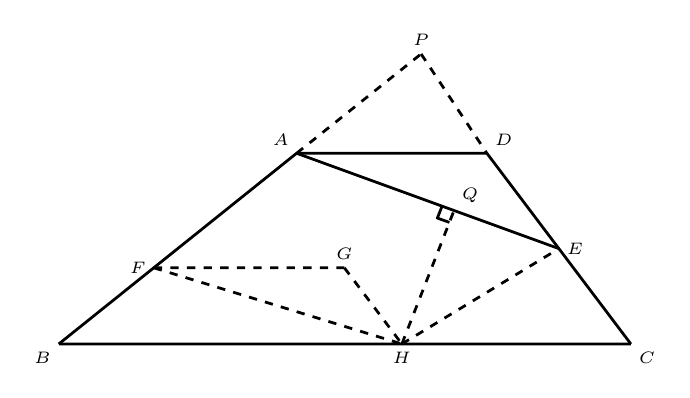
\begin{tikzpicture}[line width=1.0pt, line join=round]
% Coordinates: s = 0.008538 cm/px, origin at image point (543.5, 325)
\coordinate (B) at (-3.63181690216944,-1.817706032492616);
\coordinate (C) at (3.6339276654004173,-1.8176027853592258);
\coordinate (H) at (0.7258569238804706,-1.8176441094059168);
\coordinate (A) at (-0.6113033414360348,0.6044225588707326);
\coordinate (D) at (1.805327714727694,0.6044568994984123);
\coordinate (E) at (2.719616097699486,-0.6065575883423976);
\coordinate (F) at (-2.4249802013209534,-0.8499521656561495);
\coordinate (G) at (-0.004754439806220312,-0.8499177739472601);
\coordinate (Q) at (1.388079596230419,-0.12246774527277599);
\coordinate (P) at (0.9700468867941614,1.8659687421071969);

% Solid segments
\draw (B) -- (C);
\draw (B) -- (A);
\draw (A) -- (D);
\draw (A) -- (E);
\draw (D) -- (C);

% Dashed segments
\draw[dashed] (A) -- (P);
\draw[dashed] (P) -- (D);
\draw[dashed] (F) -- (G);
\draw[dashed] (G) -- (H);
\draw[dashed] (F) -- (H);
\draw[dashed] (H) -- (E);
\draw[dashed] (H) -- (Q);

% Right-angle mark at Q (one mark only)
\draw (1.2360999769999792,-0.06741255741763788) -- (1.1763506876638208,-0.21851047413972352) -- (1.3293296644067276,-0.2735657742890264);

% Labels
\fontsize{6}{7.2}\selectfont
\node[above left] at (A) {$A$};
\node[above right] at (D) {$D$};
\node[above] at (P) {$P$};
\node[right] at (E) {$E$};
\node[left] at (F) {$F$};
\node[above] at (G) {$G$};
\node[above right] at (Q) {$Q$};
\node[below] at (H) {$H$};
\node[below left] at (B) {$B$};
\node[below right] at (C) {$C$};
\end{tikzpicture}
\end{document}
% GEOAGENT_REPAIR_V1 c18a466396f54661 591caf6103155c450a0c23d82ae8a81e1747975d03ac2be1e2648155d2eccec1
